\documentclass[a4paper,14pt]{extarticle}
\usepackage[utf8]{inputenc}
\usepackage[russian]{babel}
\usepackage{graphicx}
\usepackage[top=0.8in, bottom=0.8in, left=0.8in, right=0.8in]
{geometry}
\usepackage{pgfplots}
\usepackage{amsmath}
\usepackage{setspace}
\usepackage{titlesec}
\usepackage{float}
\usepackage{chngcntr}
\usepackage{pgfplots}
\usepackage{amsfonts}
\usepackage{pgfplotstable}
\usepackage{multirow}
\usepackage{karnaugh-map}
\usepackage{tikz,xcolor}
\usepackage{indentfirst} % Красная строка
\usepackage{listings}
\usepackage{amssymb}
\usepackage{xcolor}
\usepackage{hyperref}

\definecolor{linkcolor}{HTML}{0000FF} % цвет ссылок
\definecolor{urlcolor}{HTML}{FF00FF} % цвет гиперссылок

\hypersetup{pdfstartview=FitH, linkcolor=linkcolor,urlcolor=urlcolor, colorlinks=true}


\titleformat{\section}[hang]
  {\bfseries}
  {}
  {0em}
  {\hspace{-0.4pt}\large \thesection\hspace{0.6em}}
  
  
\titleformat{\subsection}[hang]
  {\bfseries}
  {}
  {0em}
  {\hspace{-0.4pt}\large \thesubsection\hspace{0.6em}}

%\linespread{1.3} % полуторный интервал
%\renewcommand{\rmdefault}{ftm} % Times New Roman

\newcommand{\nx}{\overline{x}}
\newcommand{\p}{0.31}
\newcommand{\scale}{1.4}

\counterwithin{figure}{section}
\counterwithin{equation}{section}
\counterwithin{table}{section}

\begin{document}
\begin{titlepage}
\centering
Санкт-Петербургский политехнический университет Петра Великого \\
\vspace{0.15cm}
Кафедра компьютерных систем и программных технологий \\
\vspace{6.5cm}

{\centering \textbf{Отчёт по лабораторной работе} \\ 
\vspace{0.15cm}
\textbf{Дисциплина}: Телекоммуникационные технологии \\
\vspace{0.15cm}
\textbf{Тема}: Помехоустойчивое кодирование.} \\


\vspace{6.5cm}

\begin{table}[H]
\begin{tabular}{p{\textwidth}@{}r}
{Выполнил студент гр. 33501/2} \hfill {Вахаев И.Н.} \\
{Преподаватель} \hfill {Богач Н.В.} \\
\end{tabular}
\end{table}
\vfill

{\centering Санкт-Петербург \\ 
\vspace{0.15cm}
\today}
\end{titlepage}

\tableofcontents

\newpage

\section{Цель работы}

Изучение методов помехоустойчивого кодирования и сравнение их свойств.

\section{Постановка задачи}

\begin{enumerate}
\item Провести кодирование/декодирование сигнала, полученного с помощью функции randerr кодом Хэмминга 2-мя способами: с помощью встроенных функций encode/decode, а также через создание проверочной и генераторной матриц и вычисление синдрома. Оценить корректирующую способность кода.

\item Выполнить кодирование/декодирование циклическим кодом, кодом БЧХ, кодом Рида-Соломона. Оценить корректирующую способность кода.


\end{enumerate}

\section{Теоретический раздел}

\textbf{Помехоустойчивое кодирование}
Существенно сократить избыточность в передаваемых сообщения позволяет помехоустойчивое кодирование. В общем плане помехоустойчивое кодирование можно понимать как такое кодирование сообщений, при котором элементы связаны определенной зависимостью, позволяющей при ее нарушении указать ошибки и восстановить информацию. Помехоустойчивые коды рассчитаны на определенные ошибки. Это значит, что при других ошибках они могут оказаться недостаточно эффективными.	

Сообщения по каналу связи передаются в виде кодограммы. Кодограммой, или кодовой комбинацией, называется упорядоченный набор k элементов, каждый из которых может принимать m значений.
Множество всех кодовых комбинаций, поставленных в соответствие сообщениям, называется k-разрядным кодом с основанием m. Таким образом, код - множество кодовых комбинаций, а не одна комбинация.

Коды могут быть:
\begin{enumerate}

\item Безызбыточными - комбинации ставятся в соответствие каким-то сообщениям. В безызбыточном коде искажение любого элемента приводит к перерождению кодовой комбинации, т.е. изменению смыслового содержания сообщения.
\item Избыточными - использованы не все возможные комбинации. В этих кодах искажение элемента не всегда приводит к искажению сообщения. ( Так, при использовании двоичного кода в случае приема комбинации 1100 неизвестно, какая цифра передана, но и ошибки в распознавании не происходит, так как такой комбинации в коде нет. Ошибка в этом случае обнаруживается. Скорее всего переданы комбинации 1000 или 0100, поскольку они "ближе" к принятой.) Пример избыточного кодирования показан в вышеприведенной таблице.
\end{enumerate}

Идея помехоустойчивого кодирования заключается как раз в таком разнесении кодовых комбинаций, за счет введения избыточности, при котором искажения элементов не приводит к перерождению комбинаций. 

Избыточные коды иногда называют корректирующими.
Корректирующую способность оценивают минимальным кодовым расстоянием, которое жестко связано с числом исправляемых или обнаруживаемых ошибок. Минимальное кодовое расстояние - это число разрядов, по которым отличаются кодовые комбинации. Обозначается d.


\textbf{Коды Хэмминга}

Код Хэмминга - наиболее известный из первых самоконтролирующихся и самокорректирующихся кодов. Построен применительно к двоичной системе счисления. Позволяет исправлять одиночную ошибку (ошибка в одном бите) и находить двойную. Построение кодов Хэмминга основано на принципе проверки на четность числа единичных символов: к последовательности добавляется такой элемент, чтобы число единичных символов в получившейся последовательности было четным.

\textbf{Циклические коды}

Циклический код - линейный, блочный код, обладающий свойством цикличности, то есть каждая циклическая перестановка кодового слова также является кодовым словом. Используется для преобразования информации для защиты её от ошибок. Циклические коды незаменимы при необходимости передавать информацию в каналах связи, в которых отсутствует возможность повторной передачи данных. Циклические коды применяются при записи и считывании на HDD, CD и DVD, при использовании USB-портов для обмена информацией, при передаче аудио и видео информации. Среди всего многообразия групповых кодов можно выбрать такие, у которых строки связаны условием цикличности, т.е. все строки матрицы могут быть получены циклическим сдвигом одной строки, которая называется образующей или производящей. Сдвиг осуществляется справа налево, а крайний левый символ перемещается в конец строки, т.е. в крайнее правое положение. Коды, у которых строки матрицы удовлетворяют этому условию, называются циклическими.

\textbf{Коды БЧХ}

Коды Боуза — Чоудхури — Хоквингема (БЧХ-коды) — в теории кодирования это широкий класс циклических кодов, применяемых для защиты информации от ошибок. Отличается возможностью построения кода с заранее определёнными корректирующими свойствами, а именно, минимальным кодовым расстоянием. Частным случаем БЧХ-кодов является код Рида — Соломона. БЧХ-код является циклическим кодом, который можно задать порождающим полиномом. Для его нахождения в случае БЧХ-кода необходимо заранее определить длину кода и требуемое минимальное расстояние.

\textbf{Коды Рида-Соломона}

Коды Рида — Соломона — недвоичные циклические коды, позволяющие исправлять ошибки в блоках данных. Элементами кодового вектора являются не биты, а группы битов (блоки). Очень распространены коды Рида — Соломона, работающие с байтами (октетами).
Код Рида — Соломона является частным случаем БЧХ-кода.
В настоящее время широко используется в системах восстановления данных с компакт-дисков, при создании архивов с информацией для восстановления в случае повреждений, в помехоустойчивом кодировании.

\textbf{Свёрточный код}

Сверточные коды это коды, исправляющие ошибки, которые используют непрерывную, или последовательную, обработку информации короткими фрагментами (блоками). Сверточный кодер обладает памятью в том смысле, что символы на его выходе зависят не только от (очередного фрагмента) информационных символов на входе, но и предыдущих символов на его входе. Другими словами, кодер представляет со­бой последовательную машину или автомат с конечным числом состояний. Состояние кодера определяется содержимым его памяти.

\newpage
\section{Ход работы}

\subsection{Код Хэмминга}

С помощью встроенных функций encode/decode произведём кодирование/декодирование сигнала кодом Хэмминга.
Код Matlab представлен на рисунке \ref{1}.

\begin{figure}[H]
\center{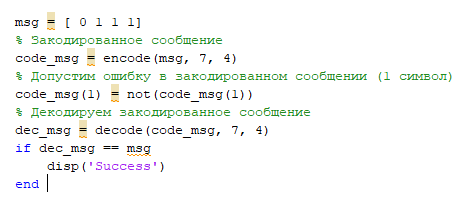
\includegraphics[width=1\linewidth]{screen/1}}
\caption{Код Matlab}
\label{1}
\end{figure}

В результате нашего кода заданный сигнал был сначала закодирован, затем в нём была допущена одна ошибка в первом символе, после чего с помощью встроенной функции decode закодированный сигнал с ошибкой был успешно декодирован, в следствие чего мы получили исходное сообщение [0 1 1 1]. Вывод программы представлен на рисунке \ref{2}

\begin{figure}[H]
\center{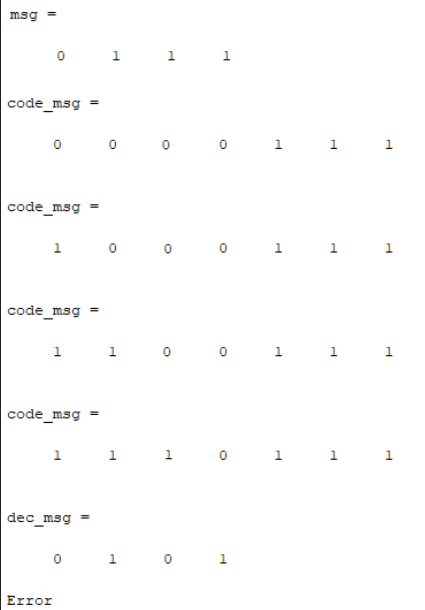
\includegraphics[width=1\linewidth]{screen/2}}
\caption{Резлуьтат выполнения программы}
\label{2}
\end{figure}

Если убрать ошибку в закодированном сигнале, то мы всё равно получим исходное сообщение. Конечный результат выполнения программы не изменится.
Если же сделать несколько ошибкой в закодированном сигнале, то код Хэмминга сумеет исправить лишь одну из них. Пример программы с несколькими ошибками приведён на рисунке \ref{3}.

\begin{figure}[H]
\center{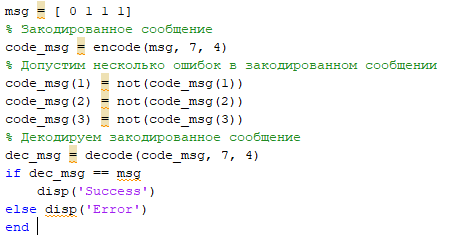
\includegraphics[width=1\linewidth]{screen/3}}
\caption{Изменённая программа в Matlab}
\label{3}
\end{figure}

Результат выполнения изменённой программы приведён на рисунке \ref{4}.
\begin{figure}[H]
\center{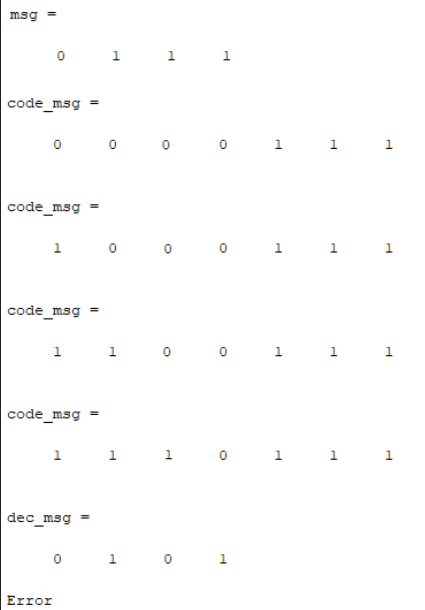
\includegraphics[width=1\linewidth]{screen/4}}
\caption{Результат изменённой программы}
\label{4}
\end{figure}

Как видно, в результате был получен ошибочный результат, на выходе не было получено исходное сообщение. Это следствие из-за большого количества ошибок в закодированном сообщении. 

Произведём кодирование/декодирование входного сигнала кодом Хэмминга путём создания генераторной и проверочной матриц, а также вычисление синдрома.

Код, реализующий это, представлен на рисунке \ref{5}

\begin{figure}[H]
\center{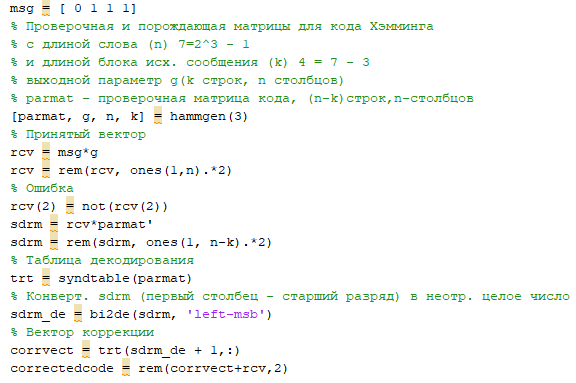
\includegraphics[width=1\linewidth]{screen/5}}
\caption{Модифицированный код в Matlab}
\label{5}
\end{figure}

При умножении исходного сообщения на генераторную матрицу в ее конечной части сохраняется исходная посылка, т.к. соответствующий блок генераторной матрицы представляет собой единичную матрицу.Оставшаяся часть формирует контрольные биты,которые составляют дополнение до нуля суммы по модулю два нужных информационных разрядов. Формирование синдрома происходит с помощью домножения на проверочную матрицу parmat'. С помощью матрицы синдрома был выявлен ошибочный бит в посылке, в нашем случае 2. Затем он был исправлен. 

Результат выполнения программы представлен на рисунке \ref{6}.

\begin{figure}[H]
\center{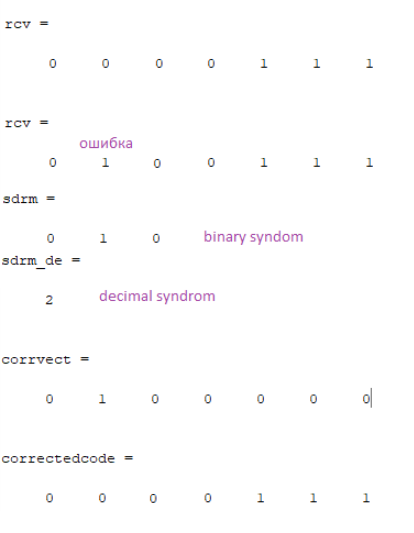
\includegraphics[width=1\linewidth]{screen/6}}
\caption{Результат выполнение кода в Matlab}
\label{6}
\end{figure}

Корректирующая способность кода равна 1

\subsection{Циклический код}

Было оставлено всё тоже сообщение [0 1 1 1]. В нём произведено кодирование/декодирование (рисунок \ref{7}):

\begin{figure}[H]
\center{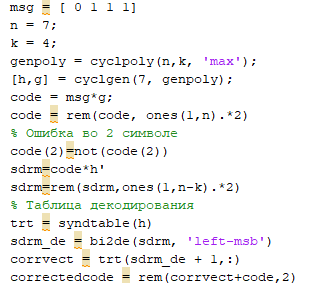
\includegraphics[width=1\linewidth]{screen/7}}
\caption{Код в Matlab}
\label{7}
\end{figure}

Был построен полином циклического кода \begin{equation} x^3 + x + 1 \end{equation}, которым использовался в качестве параметра функции cyclgen.
Были получены порождающая и проверочная матрицы. Ошибка была произведена во 2 разряде.
Результат выполнения программы представлен на рисунке \ref{8}.

\begin{figure}[H]
\center{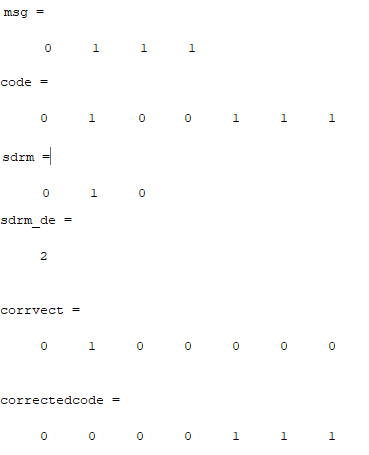
\includegraphics[width=1\linewidth]{screen/8}}
\caption{Результат выполнение кода в Matlab}
\label{8}
\end{figure}

Корректирующая способность кода равна 1

\subsection{Коды БЧХ}

Произведено кодирование/декодирование сообщения [0 1 1 1] при помощи кодов БЧХ
Данный код представлен на рисунке \ref{9}.

\begin{figure}[H]
\center{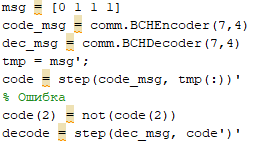
\includegraphics[width=1\linewidth]{screen/9}}
\caption{Код в Matlab}
\label{9}
\end{figure}

Результат выполнения программы показан на рисунке \ref{10}.

\begin{figure}[H]
\center{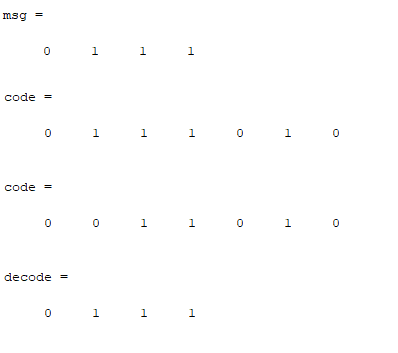
\includegraphics[width=1\linewidth]{screen/10}}
\caption{Результат выполнение кода в Matlab}
\label{10}
\end{figure}

Допущенная во 2 разряде ошибка была успешно обнаружена и исправлена, что свидетельствует о правильной работе программы.

Корректирующая способность кода равна 1. Существует возможность увеличить её до 2.

\newpage
\subsection{Коды Рида-Соломона}

Было сгенерировано три слова по три символа. Также допущены одна ошибка в первом слове, две во втором и три в третьем.
Код Matlab представлен на рисунке \ref{11}.

\begin{figure}[H]
\center{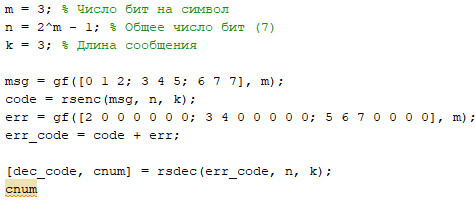
\includegraphics[width=1\linewidth]{screen/11}}
\caption{Код в Matlab}
\label{11}
\end{figure}

Результат выполнения программы представлен на рисунке \ref{12}.

\begin{figure}[H]
\center{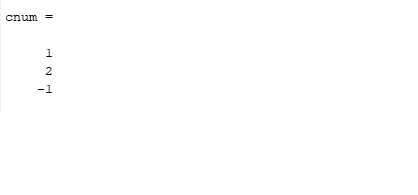
\includegraphics[width=1\linewidth]{screen/12}}
\caption{Результат выполнение кода в Matlab}
\label{12}
\end{figure}

Видно, что количество исправленных ошибок в первой и второй строке равно количеству сделанных. В третьем сообщении количество = -1, так как (7,3) RS код не может исправить более 2-х ошибок.

Из всего вышесказанного следует, что корректирующая способность кода равна 2.


\newpage

\section{Выводы}

Были рассмотрены такие методы кодирования, как: коды Хэмминга, циклические коды, коды Боуза-Чоудхури-Хоквингема и коды Рида-Соломона. Они являются самокорректирующимися. Выбор кодирования осуществляется в зависимости от поставленной задачи. По корректирующей способности коды Хэмминга уступают более сложным кодам, таким как коды БЧХ, но имеют более прозрачную реализацию. Код Рида-Соломона, в свою очередь, имеет более хороший показатель по корректирующей показатель, а так же позволяет оперировать с десятичными числами и параллельно обрабатывать несколько потоков данных. Корректирующая способность циклического кода определяется видом образующего многочлена.


\end{document}